% Number 760
% CoEM pTM CopM Algebra Units Vectors
% Cart collision - graphs, energy conservation
% AP.JG

% Watermark
\AddToShipoutPicture*{\BackgroundPic}

\addtocounter {ProbNum} {1}

\begin{floatingfigure}[r]{.44\textwidth}
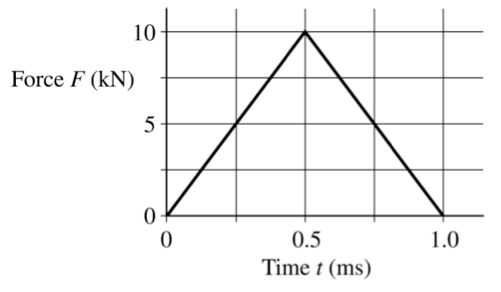
\includegraphics[scale=.5]{/Users/jgates/desktop/latex/pics/collisiongraph1}
\end{floatingfigure}
 
{\bf \Large{\arabic{ProbNum}}} A 2 kg cart is moving at a constant speed of ${3~\tfrac{m}{s}}$ on a horizontal surface when it collides with a second cart of mass $m$ (initially at rest). The force exerted by the moving cart on the stationary cart is shown as a function of time from the beginning of the impact. After the collision, the second cart is moving to the right at ${1.6~\tfrac{m}{s}}$.\bigskip

Determine the magnitude and direction of the velocity of the 2 kg cart after the collision. \paragraph{}
\noindent
\vfill

Determine the mass of the target cart.
\vfill

\begin{floatingfigure}[r]{.45\textwidth}
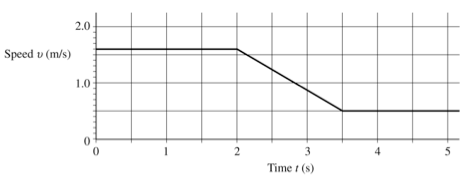
\includegraphics[scale=.55]{/Users/jgates/desktop/latex/pics/collisiongraph2}
\end{floatingfigure}
After the collision, the target cart encounters a frictionless ramp. The speed of the cart during the five seconds after the collision is shown.

\bigskip
Did the ramp go up or down? Determine the elevation of the end of the ramp (height gained or lost, measured from the initial track's level).

\vfill
\vfill
%\hfill 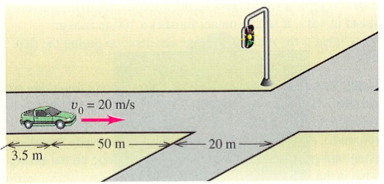
\includegraphics[scale=.85]{/Users/jgates/desktop/latex/pics/redlight.png}
\newpage